\section{Conclusion and Future Works}

\begin{frame}{Conclusion}

\destaq{Advancements}

\begin{itemize}
    \item  Addressing the Last Mile Delivery Drones problem through a MAPF approach ;
    \item Ensuring collision avoidance and efficient airspace control.
    \item Significant advancement over previous algorithms with guaranteed finite and bounded polynomial time convergence for the heuristic
\end{itemize}

\bigskip

\destaq{Limitations}

\begin{itemize}
    \item Does not address real world problems like energy, fuel and speed of the drones;
    \item The experiment using binary search to find the T for the MILP in $\mathcal{O}( \log( T)$) is not conducted;
    \item Small grid sizes in experiments;
\end{itemize}

\end{frame}

\begin{frame}{Future Works}
    \begin{figure}
      \begin{columns}
        \column{.23\linewidth}
        \caption{Tradable Permit Model in the Decentralized LMDD. \\ Source: \cite{Verri}}
        \label{fig:trad_drones}
        \column{.75\linewidth}
        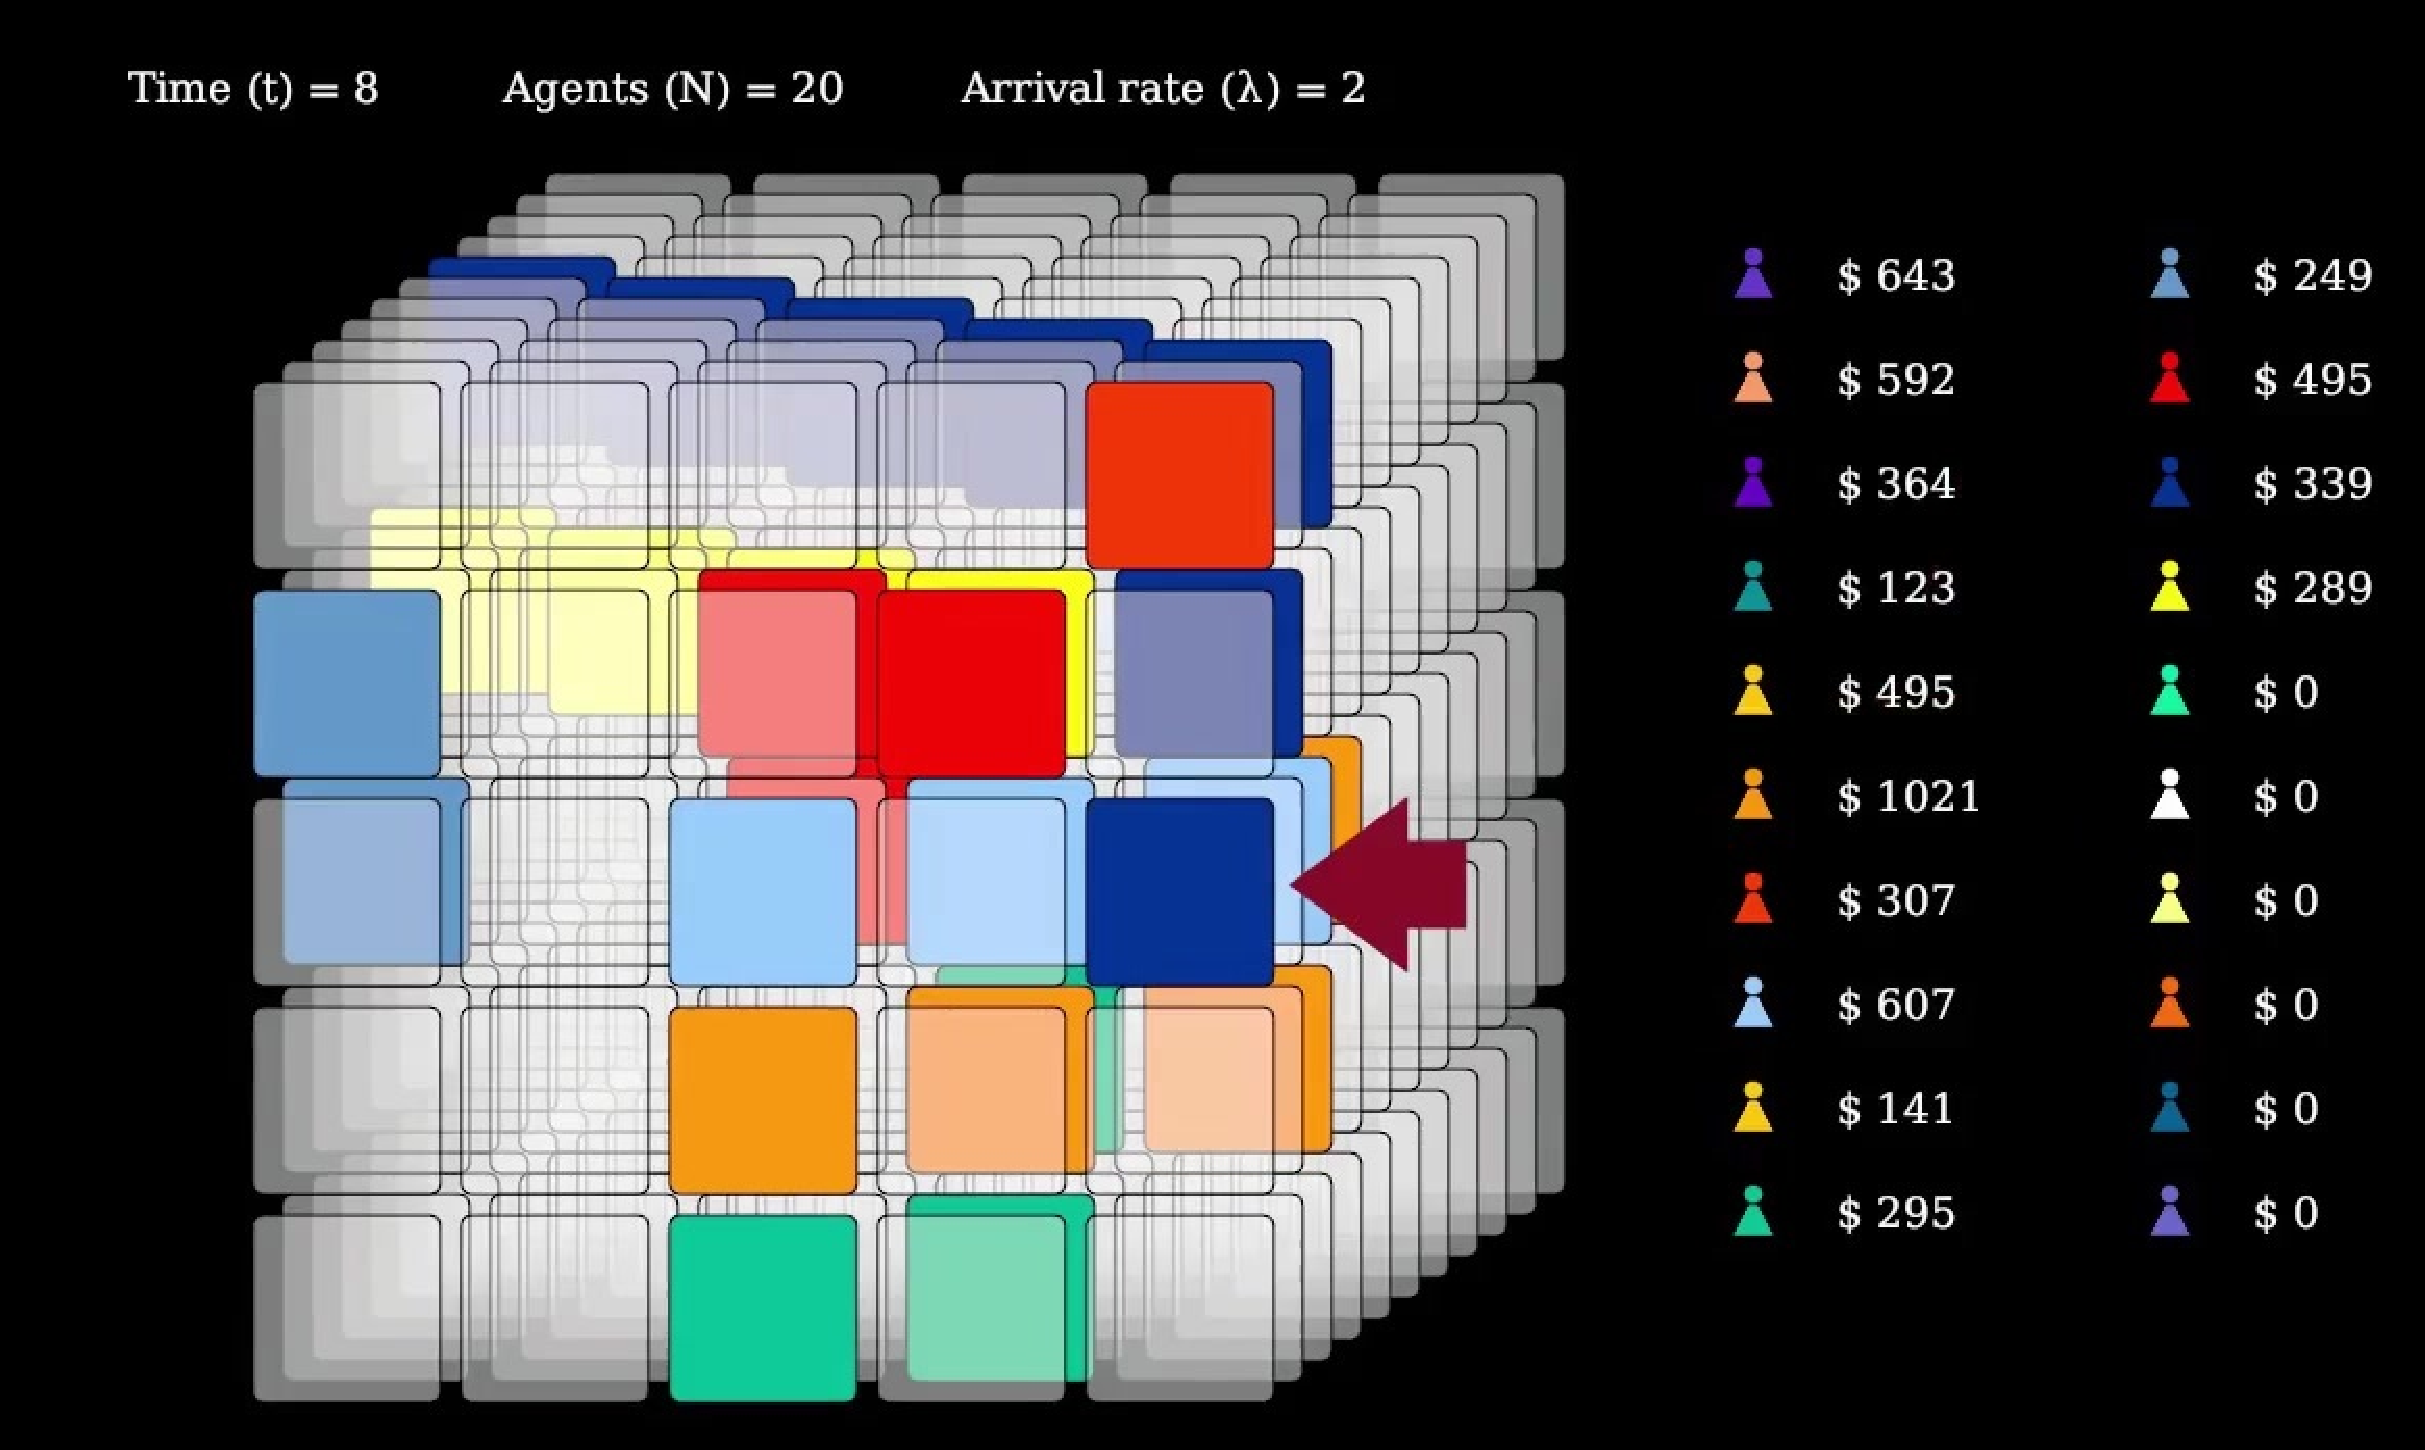
\includegraphics[width=\textwidth]{img/trad_drones-pdf-jpg-to-pdf.pdf}
      \end{columns}
    \end{figure}

\end{frame}


\begin{frame}{Future Works}
\destaq{Decentralized Model from \cite{Verri}}
\begin{itemize}
    \item naive agents
    \item greedy random choices
\end{itemize}
\bigskip
\destaq{Decentralized Model with Intelligence}
\begin{itemize}
    \item Reinforcement Learning
    \item Graph Dynamical System
    \begin{itemize}
        \item Complex Networks
        \item Graph Neural Networks
    \end{itemize}
\end{itemize}
\end{frame}
